\documentclass[12pt,letterpaper]{article}
\usepackage{amsmath}
\usepackage{amsthm}
\usepackage{amsfonts}
\usepackage{amssymb}
\usepackage{amscd}
\usepackage{enumerate}
\usepackage{fancyhdr}
\usepackage{mathrsfs}
\usepackage{bbm}
\usepackage{framed}
\usepackage{mdframed}
\usepackage{cancel}
\usepackage{mathtools}
\usepackage{verbatim}
\usepackage{hyperref}
\usepackage[letterpaper,voffset=-.5in,bmargin=3cm,footskip=1cm]{geometry}
\setlength{\parindent}{0.0in}
\setlength{\parskip}{0.1in}
\allowdisplaybreaks
\headheight 15pt
\headsep 10pt
\newcommand\N{\mathbb N}
\newcommand\Z{\mathbb Z}
\newcommand\R{\mathbb R}
\newcommand\Q{\mathbb Q}
\newcommand\lcm{\operatorname{lcm}}
\newcommand\setbuilder[2]{\ensuremath{\left\{#1\;\middle|\;#2\right\}}}
\newcommand\E{\operatorname{E}}
\newcommand\V{\operatorname{V}}
\newcommand\Pow{\ensuremath{\operatorname{\mathcal{P}}}}

\DeclarePairedDelimiter\ceil{\lceil}{\rceil}
\DeclarePairedDelimiter\floor{\lfloor}{\rfloor}
\newcommand\hint[1]{\textbf{Hint}: #1}
\newcommand\note[1]{\textbf{Note}: #1}
\newcounter{enum22i}
\newenvironment{22enumerate}{\begin{enumerate}[a.]\itemsep0em\setcounter{enumi}{\value{enum22i}}}{\setcounter{enum22i}{\value{enumi}}\end{enumerate}}
\newenvironment{22itemize}{\begin{itemize}\itemsep0em}{\end{itemize}}
\fancypagestyle{firstpagestyle} {
  \renewcommand{\headrulewidth}{0pt}
  \lhead{\textbf{CSCI 0220}}
  \chead{\textbf{Discrete Structures and Probability}}
  \rhead{M. Littman}
}

\fancypagestyle{fancyplain} {
  \renewcommand{\headrulewidth}{0pt}
  \lhead{\textbf{CSCI 0220}}
  \chead{Problem}
  \rhead{\textit{ }}
}
\pagestyle{fancyplain}
\usepackage{tikz}
\usepackage{graphicx}

\begin{document}
  \thispagestyle{firstpagestyle}
  \begin{center}
    {\huge \textbf{Homework 5}}

    {\large Due: \textit{Monday, June 21st at 11:59pm EDT}}
  \end{center}


     All homeworks are due the Monday after their release at 11:59pm EDT on Gradescope.

    Please do not include any identifying information about yourself in the handin, including your Banner ID.

    Be sure to fully explain your reasoning and show all work for full credit. We recommend checking out the sample proofs on the course website to see the level of rigor for which we're looking.



\subsection*{Problem 1}
{
\nopagebreak 

{\setcounter{enum22i}{0}

    	\begin{22enumerate}
        \item
          Prove that, provided two bijections $f: Q \to R$ and $g: R \to Q$ (where $Q$ and $R$ are non-empty), 
          the composition $f\circ g$ is a bijection. 
          % The composition is defined as $f \circ g(x) = f(g(x))$ for any $x \in R$.
        \item
          Applying an arbitrary function repeatedly to some initial value is called an {\em iterated map}. Let $f$ be a bijection $f: R \to R$. Let $g^n$ be a function $g^n: R \to R$ that applies $f$ a total of $n$ times where $n \geq 1$. That is, $g^n(x) =  f(f(f(\ldots f(x)\ldots )))$ where $f$ is applied $n$ times. Prove that $g^n$ is a bijection using induction.
      \end{22enumerate}
    
}
}



\subsection*{Problem 2}
{
\nopagebreak
\newcommand\PersonA{Phobos}
\newcommand\PersonB{Deimos}
\newcommand\objects{meteors}
\newcommand\object{meteor}

{\setcounter{enum22i}{0}

      The two moons of Mars, \PersonA\ and \PersonB\, have been stuck in tidally locked orbits for millions of years. The same face of each moon points towards the planet at all times. In an effort to make staring at the surface a little more exciting, they decide to play a \textit{very fun game}.
      
      \PersonA\ gathers incoming Martian meteors and places them on the Martian surface into two separate piles of equal size. Then, at each turn \PersonA\ and \PersonB\ each remove some positive number of \objects\ from one of the piles. The player who removes the last \object\ wins. Since the game is \PersonA ' idea, it decides to go first. Prove that \PersonB\ can always win.
      
      \hint{Use strong induction!}
    
}
}



\subsection*{Problem 3}
{
\nopagebreak 

{\setcounter{enum22i}{0}

      \begin{22enumerate}

      \item
      Prove by induction that for all positive integers $n$, there exists a positive integer $m$ such that:
      \[m^2 \leq n < (m + 1)^2\]

      \item
      Prove by contradiction that there exists a \textbf{unique} such $m$.

      \end{22enumerate}
    
}
}


\subsection*{Mind Bender (Extra Credit)}
{
\nopagebreak 

{\setcounter{enum22i}{0}
  \begin{22enumerate} 
   \item Consider the figure below.
   \begin{center}
  \begin{tabular}{cc}
    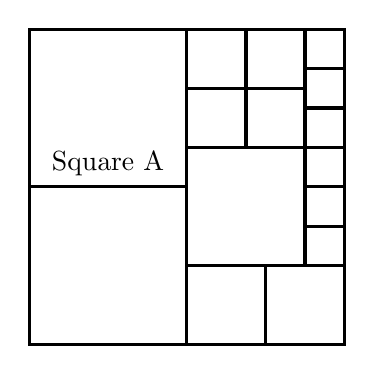
\begin{tikzpicture}
      \draw [-,very thick,black] (0,-2) -- (-2,-2) -- (-2,2) -- (1.5,2) -- (2,2) -- (2,1.5) -- (1.5,1.5) -- (1.5,2) -- (1.5,1.5) -- (2,1.5) -- (2,-2) -- (0,-2) -- (0, -2) -- (0, 0) -- (-2, 0);
      \draw [-,very thick,black] (0,2) -- (0,0);
      \draw [-,very thick,black] (1.5,1.5) -- (1.5,-1);
      \draw [-,very thick,black] (0,0.5) -- (2,0.5);
      \draw [-,very thick,black] (1.5,1) -- (2,1);
      \draw [-,very thick,black] (0.75,0.5) -- (0.75,2);
      \draw [-,very thick,black] (0,1.25) -- (1.5,1.25);
      \draw [-,very thick,black] (0,-1) -- (2,-1);
      \draw [-,very thick,black] (1.5,0) -- (2,0);
      \draw [-,very thick,black] (1.5,-0.5) -- (2,-0.5);
      \draw [-,very thick,black] (1,-1) -- (1,-2);
      \draw [-,very thick,black] (-1.9,0) -- node[above=0pt] {Square A} (-0.1,0);
    \end{tikzpicture}\\
  \end{tabular}
  \end{center}
  How does the number of non-overlapping squares in the figure change if Square A is subdivided into squares whose side lengths are half that of the original's?  To give you a sense of what counts as a non-overlapping square, the figure initially has 15 non-overlapping squares.
   \item Divide the square below into exactly 6 (not necessarily congruent) squares such that there is no overlap and the entire region is covered.
  \begin{center}
  \begin{tabular}{cc}
    
\begin{tikzpicture}
      \draw [-,very thick,black] (-2,-2) -- (-2,2) -- (2,2) -- (2,-2) -- (-2,-2);
    \end{tikzpicture}\\
  \end{tabular}
  \end{center}
  
   \item Prove by induction that every integer greater than 5 can be written in the form $a + 3m$, where $a$ is 6, 7, or 8, and
   $m$ is a non-negative integer.
    
   \item Using parts (a), (b), and (c) for inspiration, prove by induction that a square can be subdivided into \emph{n} (not necessarily congruent) squares such that there is no overlap and the entire region is covered for all integral \emph{n} greater than 5.
   
   \textbf{Note: }You may assume that your answer to (a) is correct.
  \end{22enumerate}
}
}



\end{document}